\chapter{Avaliação Experimental} \label{Cap:Ava_Exp}
4.1 Validação Técnica da Comunicação entre Camadas
\subsection{Validação Funcional da Web API}

Nesta etapa, realizou-se um teste funcional para validar se a Web API .NET 9 conseguia orquestrar corretamente a requisição entre o orquestrador (Semantic Kernel) e o modelo de linguagem na nuvem (Azure OpenAI). O teste foi realizado utilizando a interface Swagger UI.

A Figura \ref{fig:resposta_api} apresenta a resposta JSON obtida para uma pergunta simulada sobre a tela de "Cadastro de Lotes".

\begin{figure}[H]
    \centering
    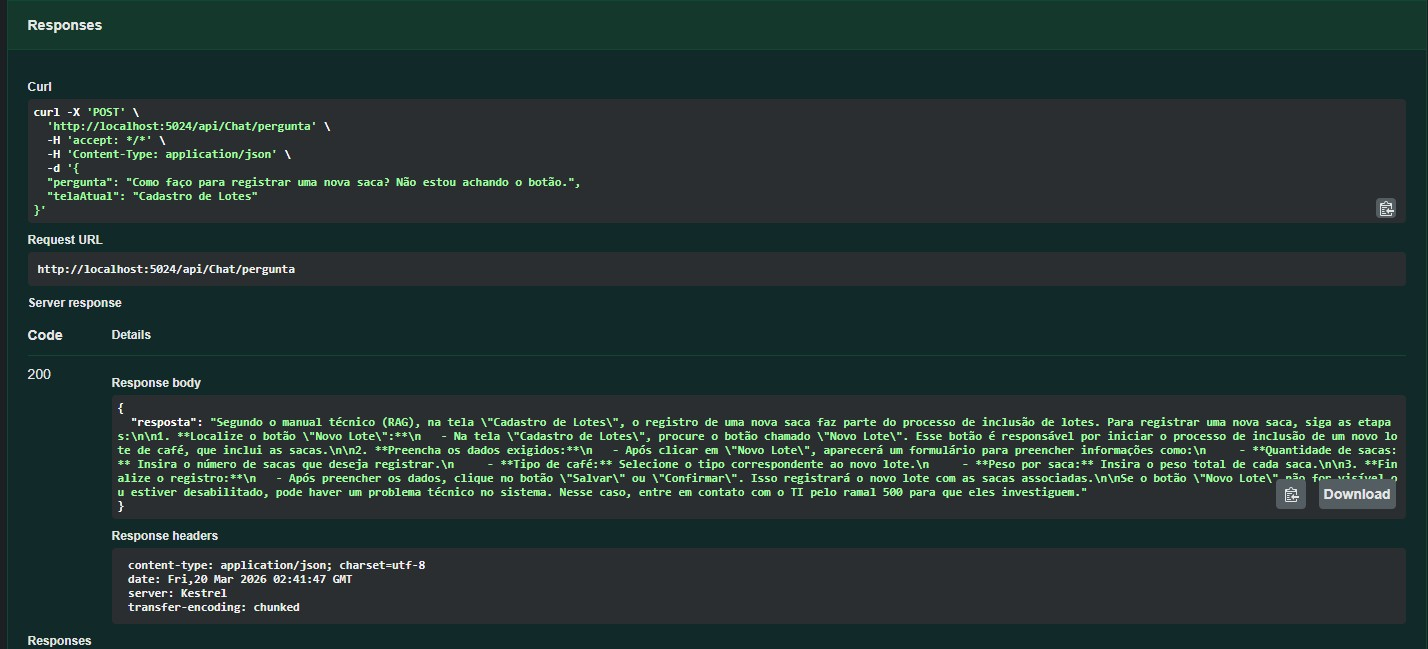
\includegraphics[width=0.8\textwidth]{USPSC-img/ValidacaoInicial-API.jpg}
    \caption{Evidência de resposta bem-sucedida da API integrando prompt dinâmico e contexto de tela.}
    \label{fig:resposta_api}
\end{figure}

Pode-se observar que a resposta gerada pela IA respeitou as diretrizes de persona e contingência estabelecidas, incluindo a orientação para contato com o TI no ramal 500 caso persistissem dificuldades técnicas. Isso valida a 'plumbagem' tecnológica do sistema.